\graphicspath{ {./images/6_Protein_quantitation} }
\newpage

\section{Protein quantitation (optional)}
This option can be used when the samples contain one or more stable isotope labeled standards, such as SILuMAb for quantitation of antigen-specific IgG1.\footnote{See our technical note for details: \url{https://pubs.acs.org/doi/10.1021/acs.jproteome.4c00538}}

A \texttt{.xlsx} file containing the following columns is required:
\begin{itemize}[topsep=0pt, itemsep=0pt]
	\item \textsf{protein} - Name of the protein to be quantified using the natural/labeled pair.
	\item \textsf{natural} - Name of the natural glycosylation site (when quantifying based on glycopeptides), or the name of a natural non-glycosylated peptide \emph{as detected by GlycoDash} (see \nameref{data_import}).
	\item \textsf{labeled} - Name of the stable isotope labeled glycosylation site (when quantifying based on glycopeptides), or of the labeled non-glycosylated peptide \emph{as detected by GlycoDash} (see \nameref{data_import}).
	\item \textsf{standard\_ng} - The absolute amount of stable isotope labeled standard that was added to each sample, in nanograms (ng).
	This amount is assumed to be identical for all samples.
	\item \textsf{sample\_ul} - The volume of sample from which the proteins were isolated, in microliters ($\textmu$L). 
	This volume is assumed to be identical for all samples.
\end{itemize}

\begin{examplebox}
	Below is a screenshot of an example \texttt{.xlsx} file.
	\begin{center}
		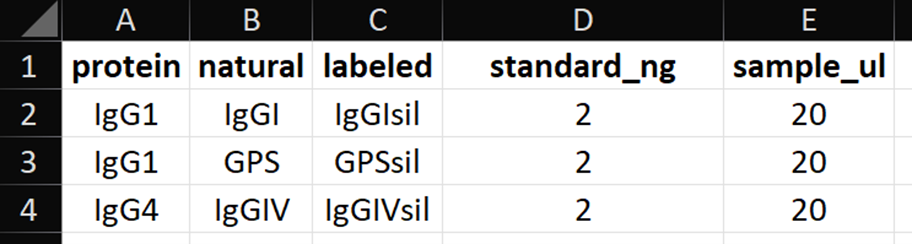
\includegraphics[scale=0.35]{example.png}
	\end{center}
	Here two proteins were quantified:
	\begin{itemize}[topsep=0pt, itemsep=0pt]
		\item \textsf{IgG1} was quantified based on glycopeptides and based on a non-glycosylated peptide.
		\begin{itemize}
			\item \textsf{IgGI} was the glycosylation site of natural \textsf{IgG1} glycopeptides.
			\textsf{IgGIsil} was the name of the glycosylation site of the labeled \textsf{IgG1} glycopeptides.
			\item \textsf{GPS} was the name of a natural non-glycosylated peptide, and \textsf{GPSsil} was the name of the corresponding labeled peptide.
		\end{itemize}
		\item \textsf{IgG4} was quantified based solely on glycopeptides, \textsf{IgGIV} representing the natural glycopeptides and \textsf{IgGIVsil} representing the labeled glycopeptides.
	\end{itemize}
\end{examplebox}

Quantitation using glycopeptides is based on the sum intensity ratio between the natural glycopeptides and the labeled glycopeptides.
Quantitation using non-glycosylated peptides is based on the intensity ratio between the natural peptide and the labeled peptide.

Quantities are reported as concentrations in the original sample in nanograms per millileter (ng/mL). 
\emph{Note that this may be a systematic underestimation if the standard is not added to the original sample but in a later step during the sample preparation.}

When more than one natural/labeled pair is specified for a protein, the median quantity is reported.
In the example above, \textsf{IgG1} was quantified based on both \textsf{IgGI/IgGIsil} and \textsf{GPS/GPSsil} ratios, giving two different quantities for each sample.
The reported quantity is the median of these two quantities.

\newpage
Correlation plots between the quantities based on the different pairs are generated, including a line of equality ($y = x$).
The closer data points are to this line, the more the two quantity calculations are in agreement.
Ideally, there should be a good correlation.
Otherwise, we suggest to investigate the validity of each natural/labeled pair.

Non-glycosylated peptides are not considered during spectral curation and analyte curation.
When non-glycosylated peptides are used for quantitation of a protein, the percentage of samples in which the peptide ions fulfill the three quality criteria is plotted.
For $S/N$ and IPQ (in the case of LaCyTools or SweetSuite data), or total area and IDP (Skyline data), the same criteria that were used for spectra and analyte curation are applied.
Because non-glycosylated peptides are often quantified without spectrum calibration, you may want to be more lenient when it comes to the acceptable mass error.
This acceptable mass accuracy range can therefore be set manually.
There is also an option to exclude sample types (e.g., blanks and negative controls) from the quality assessment.

\begin{center}
	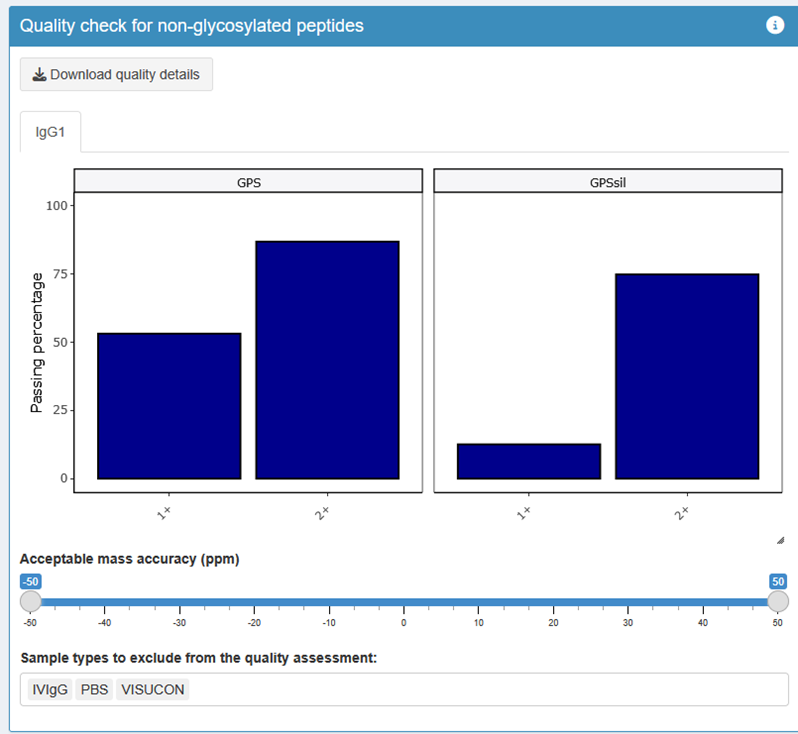
\includegraphics[scale=0.7]{peptide_qc.png}
\end{center}

If you conclude that a certain peptide or one of its charge states is of insufficient quality, it can be excluded from being used for quantitation under \textsf{Non-glycosylated peptide ions to exclude from the calculations}.





